Um Audio Deepfakes erstellen zu können gibt es verschiedene Tools, für die verschiedene Arten des Audio Deepfakes.
In dieser Arbeit werden wir auf 2 unterschiedlichen Audio Deepfake Tools eingehen, um die vielfältigkeit der Deepfake besser demonstrieren zu können.
Hierfür verwenden wir das Tool Tacotron2, für einen Text to Speech Deepfake und das Tool Real-Time Voice Cloning, um eine Echtzeit Sprachklonung durchzuführen.

\section{Tacotron2}
Tacotron ist eine Architektur für Sprachsynthesen, die eine \gls{Sequenz-zu-Sequenz-Methode} verwendet, um \gls{Magnituden-Spektrogramme} direkt aus einer Eingabesequenz von Zeichen zu erzeugen.

\subsection{Motivation}
Die Motivation hinter Tacotron2 ist es bei der Erstellung von Text-to-Speech Deepfakes die Sprachqualität deutlich zu verbessern, sodass die synthetisch generierte Sprache so natürlich wie mie möglich klingt.
Außerdem reduziert Tacotron2 die Komplexität des Prozesses, welcher normalerweise viel Fachkenntnisse und manuelle Anpassungen benötigt.\cite{Arxiv},\cite{Arxiv2}

\subsection{Fähigkeiten}
Tacotron2 zeichnet sich durch mehrere Hauptmerkmale aus:
\begin{itemize}
    \item \textbf{Sequenz-zu-Sequenz Modell:} Dieses Modell wird verwendet, um die Eingabesequenz (Text) in eine Ausgabesequenz (Sprachspektrogramm) zu konvertieren. Das Modell verwendet außerdem Aufmerksamkeitsparadigmen, um dem Modell zu helfen, sich auf relevante Teile des Textes zu konzentrieren, während es die Sprache generiert.\cite{Arxiv2}
    \item \textbf{Mel-Spektrogramm Generierung:} Diese Spektrogramme, bieten die Möglichkeit als Eingabe für ein Vocoder verwendet zu werden, welches die endgültige Audiosynthese durchführen kann, um noch bessere Audioqualität zu erreichen.\cite{Arxiv}
    \item \textbf{Flexibilität:} Tacotron2 ist in der Lage, verschiedene sprachliche Eigenschaften und Stile zu erlernen und wiederzugeben, wodurch es eine breite Auswahl zur Generierung von Stimmen und Ausdrucksweisen hat.\cite{Arxiv}
    \item \textbf{Integration mit Vocoder:} Tacotron2 übernimmt die Generierung der Spektrogramme, welche dann optimal in ein Vocoder, wie z.B. WaveNet, eingegeben werden kann, um so die finale Sprachsynthese durchführen zu können. Zudem führt die Kombination aus Tacotron2 und einem Vocoder zu einer deutlich verbesserten Audioqualtität, weshalb die Integration mit einem guten Vocoder von hoher Bedeutung ist. \cite{Arxiv}
\end{itemize}

\subsection{Workflow}
Der Workflow von Tacotron2 ist in einer Pipeline und besteht aus drei Hauptphasen: Extraction, Training und Conversion.
\subsubsection*{Pretraining}
Für die Erstellung eines Deepfakes wird eine Sammlung von Daten benötigt, um das Modell trainieren zu können. Die Sammlung beinhalten das Zusammenstellen eines Datensatzes aus Text- und Sprachaufnahmen. Hierbei wird darauf geachtet das die Daten für das Training des Modells geeignet sind.\cite{Arxiv}
\subsubsection*{Extraction}
In der Extraktionsphase werden dann die relevanten Abschnitte aus den Sprachaufnahmen extrahiert. Tacotron2 wandelt hierbei die Sprachaufnahmen in Mel-Spektrogramme um, die das Modell anschließend dann während des Trainings verwendet.\cite{Arxiv}
\subsubsection*{Training}
Durch das Training passiert dann der eigentliche Prozess, in der ein Modell trainiert wird, um realistische Text-To-Speech Ausgaben zu erzeugen. Dabei wird das Modell darauf trainiert, aus den Eingabetexten Mel-Spektrogramme zu erzeugen. Parallel oder auch anschließend dazu kann ein Vocoder, wie WaveNet, trainiert werden, um aus den Mel-Spektrogrammen die endgültige Audiodaten zu erzeugen.\cite{Arxiv}
\subsubsection*{Conversion}
In der letzten Phase, die Konvertierungsphase, werden dann die Spektrogramme in eine Wellenform umgewandelt. Der Prozess von der Erzeugung von Sprache aus einem Spektrogramm wird Vocoder genannt. Dadurch wird dann die tatsächliche Sprache generiert.\cite{Arxiv},\cite{pytorch}
\section{Praxisbeispiel Tacotron2}
Im Folgenden wird der Workflow zum Erstellen von Audio (Text-To-Speech) Deepfakes mit Tacotron näher betrachtet. Ziel dieses Kapitels ist es eine menschliche Audiodatei von einer Texteingabe zu erzeugen.
\subsection{Laborumgebung}
Die Tacotron2 Audio Deepfakes werden auf folgender Hardware erstellt.\\[0.5cm]
\begin{tabular}{rl}
    CPU:& \texttt{AMD Ryzen 7 2700X}\\
    RAM:& \texttt{16GB DDR4 3000MHz}\\
    GPU:& \texttt{NVIDIA GTX 1070 (8GB GDDR5)}\\
    OS:& \texttt{Windows 10}\\
    Mikrofon:& \texttt{Auna Mic CM900}\\
    Aufnahmeprogramm:& \texttt{Audacity}
\end{tabular}\\[0.5cm]
\subsection{Programmstruktur}
Für Vorbereitung und Pretraining des Trainingsmaterials wurden folgende 3 Skripts verwendet:
\begin{itemize}
    \item \textbf{transcribe\_wav2vec.py:} Das Skript \href{https://github.com/rasmurtech/Tacotron2-Wav2Vec-Transcription}{transcribe\_wav2vec.py} wird verwendet, um grobe Transkripte von den Aufnahmen zu erstellen. Dieses Transkript kann auch händisch geschrieben werden, jedoch erspart dieses Skript eine Menge Zeit.
    \item \textbf{tacotron2\_preprocessor\_wav\_files.py:} Das Skript \href{https://github.com/rasmurtech/Tacotron-2-Audio-Preprocessor}{tacotron2\_preprocessor\_wav\_files.py} wird verwendet, um die Audiodateien in das von Tacotron2 benötigte Format zu konvertieren.
    \item \textbf{audio\_metadata\_updater.py:} Das Skript \href{https://github.com/rasmurtech/Audio-Metadata-Updater}{audio\_metadata\_updater.py} wird verwendet, um den Titel jeder WAV Datei zu aktualisieren, sodass er der entsprechenden Nummer entspricht. Auch dieses Skript wird nicht dringen benötigt, da der Vorgang auch händisch getan werden kann. Jedoch spart es auch hier eine Menge an Zeit.
\end{itemize}
Für das anschließende Training und Synthetisieren der Modelle werden folgende 2 Ipynb Dateien verwendet:
\begin{itemize}
    \item \textbf{FakeYou\_Tacotron\_2\_Training.ipynb:} \href{https://colab.research.google.com/github/justinjohn0306/FakeYou-Tacotron2-Notebook/blob/dev/FakeYou_Tacotron_2_Training.ipynb}{Hier} wird das Training der Modelle konfiguriert und ausgeführt.
    \item \textbf{FakeYou\_Tacotron2\_Hi\_Fi\_GAN\_(CPU).ipynb:} \href{https://colab.research.google.com/github/justinjohn0306/FakeYou-Tacotron2-Notebook/blob/main/FakeYou_Tacotron2_Hi_Fi_GAN_(CPU).ipynb}{Hier} werden die trainierten Modelle synthetisiert und ausgegeben.
\end{itemize}
\subsection{Vorbereitung}
Bevor der Deepfake erstellt werden kann, müssen zuvor einige Schritte durchgeführt werden. Zuerst werden Audiospuren einer Person benötigt, um genug Ausgangsmaterial für das Training später zu verfügung zu haben. Hierzu müssen mehrere verschiedene Sätze, Satz für Satz, aufgenommen und in seperate .wav Audiodateien gespeichert werden. Hierbei gilt natürlich, je mehr Audiodateien zur verfügung stehen, desto besser wird am Ende das trainierte Modell klingen. Die Audiodateien sollen dann in eine gemeinsame Ordner mit einer Zahl als Dateinamen, aufteigend, abgelegt werden (z.B. 1.wav, 2.wav, 3.wav, ...).\newline
Danach wird ein \href{https://github.com/rasmurtech/Tacotron2-Wav2Vec-Transcription/blob/main/transcribe_wav2vec.py}{Skript} benötigt, um grobe Transkripte der Aufnahmen zu erstellen. Hierbei wird eine Liste.txt Datei erstellt, in der die aufgenommenen Sätze stehen. Diese Liste muss auf Richtigkeit geprüft werden. Es sollte außerdem darauf geachtet werden, dass jede Zeile mit einem Punkt endet und weder Großbuchstaben noch Kommas im Satz vorkommen.\newline
\subsection{Pretraining}
Um das Training durchführen zu können, müssen zunächst die zuvor erstellten .wav Audiodateien durch ein preprocessing Skript durchlaufen. Das \href{https://github.com/rasmurtech/Tacotron-2-Audio-Preprocessor/blob/main/tacotron2_preprocessor_wav_files.py}{Skript} konvertiert die Audiodateien in das von Tacotron2 benötigte Format. Es ändert das Audioformat, einschließlich der Abtastrate und Kanäle.\newline
Nachdem das preprocessing erfolgreich durchlaufen ist, muss in jeder .wav Audiodatei die entsprechende Zahl als Titel eingefügt werden. Hierzu gibt es ein weiteres \href{https://github.com/rasmurtech/Audio-Metadata-Updater/blob/main/audio_metadata_updater.py}{Skript}, dass die Zahlen aufsteigend in den Titel der jeweiligen Audiodateien schreibt.\newline
Danach muss der Ordner, in den die .wav Audiodateien liegen, in einen komprimierten Zip-Ordner erstellt und dann in Google Drive hochladen werden.
\subsection{Extraktion}
\subsubsection*{Training}
Um das Modell zu trainieren wird \href{https://colab.research.google.com/github/justinjohn0306/FakeYou-Tacotron2-Notebook/blob/dev/FakeYou_Tacotron_2_Training.ipynb}{Google Colab} verwendet. Dort müssen zunächst mehrere Schritte getan werden, bevor es zum Trainieren des Modells geht. Zuerst wird die GPU überprüft, danach muss Google Drive verbunden werden und anschließend Tacotron2 installiert werden.
\begin{figure}[H]
    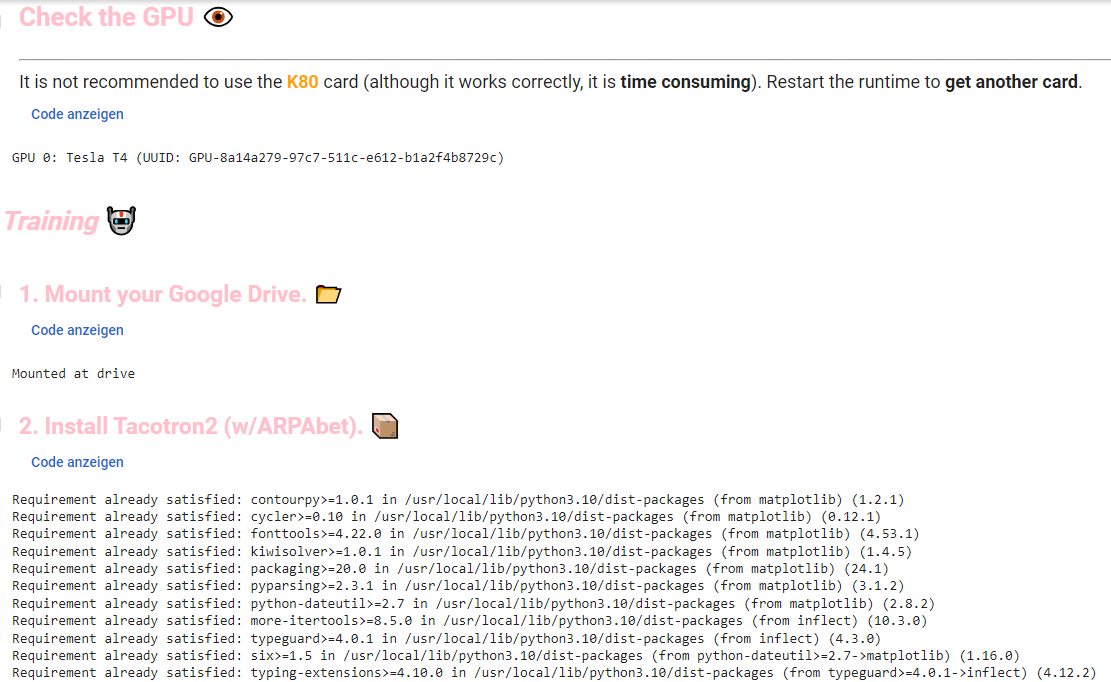
\includegraphics[width=1.0\textwidth]{Bilder/AudioTraining1}
    \centering
    \caption{GPU Prüfung, Google Drive Verbindung und Tacotron2 Installation}
    \label{fig:TrainingPart1}
\end{figure}
Nach der Installation von Tacotron2 muss die wavs.zip Datei ausgewählt werden, sowie das Transkript (list.txt), welches am Anfang erstellt wurde.
\begin{figure}[H]
    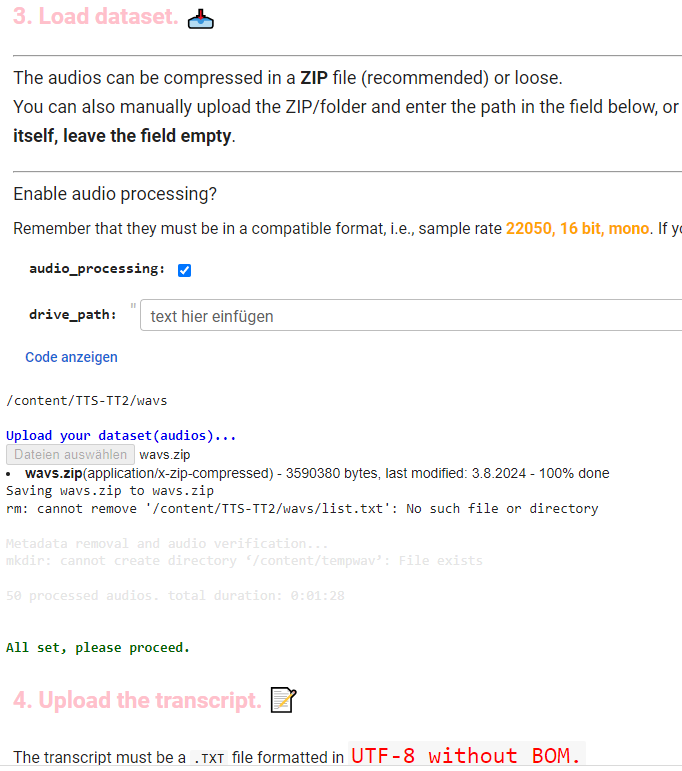
\includegraphics[width=1.0\textwidth]{Bilder/AudioTraining2}
    \centering
    \caption{Datensatz laden für Modell Training}
    \label{fig:TrainingPart2}
\end{figure}
Nach dem Hochladen des Datensatzes kann das Modell konfiguriert werden, mit welchen Parametern das Training ausgeführt werden soll.
\begin{figure}[H]
    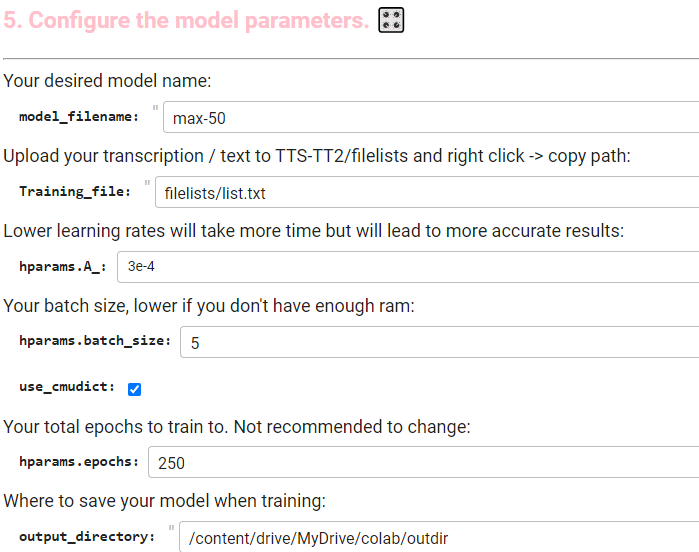
\includegraphics[width=1.0\textwidth]{Bilder/AudioTraining3}
    \centering
    \caption{Konfiguration der Modell Parameter}
    \label{fig:TrainingPart3}
\end{figure}
Danach werden die .wav Dateien in die sogenannten Mel Spektrogramme konvertiert.
\begin{figure}[H]
    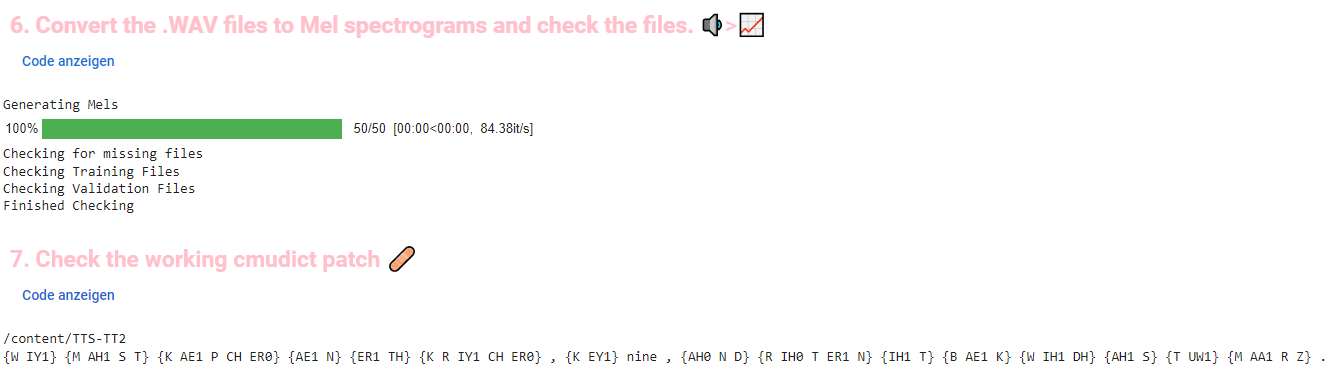
\includegraphics[width=1.0\textwidth]{Bilder/AudioTraining4}
    \centering
    \caption{Met Spektrogramme Konvertierung}
    \label{fig:TrainingPart4}
\end{figure}
Sobald die Vorbereitungen abgeschlossen sind, kann das Modell trainiert werden. Das trainierte Modell befindet sich nach dem Training in dem angegebenen Google Drive Ordner.
\begin{figure}[H]
    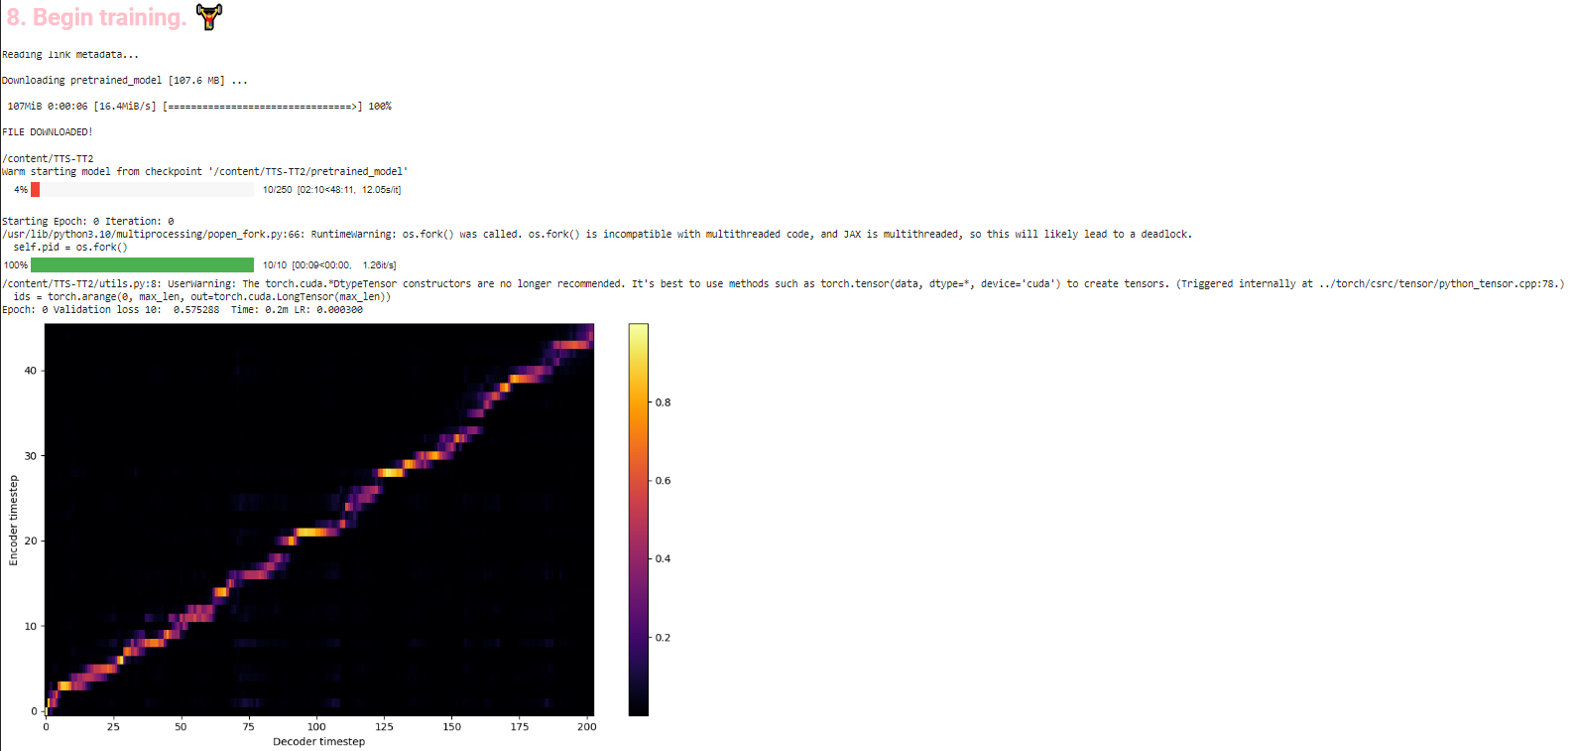
\includegraphics[width=1.0\textwidth]{Bilder/AudioTraining5}
    \centering
    \caption{Modell Training}
    \label{fig:TrainingPart5}
\end{figure}
\subsubsection*{Synthetisierung von Sprache}
Nach dem Training des Modells, muss die Sprache noch synthetisiert werden. Hierfür muss zunächst das Modell in Google Drive auf Öffentlich gestellt und danach die Tacotron ID aus dem Google Drive Link kopiert werden. Die Tacotron ID ist immer unterschiedlich von Modell zu Modell.
\begin{figure}[H]
    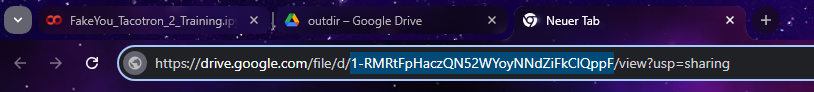
\includegraphics[width=1.0\textwidth]{Bilder/AudioTrainingLink}
    \centering
    \caption{Tacotron ID aus dem Link des Modells}
    \label{fig:TrainingLink}
\end{figure}
Danach kann die Tacotron ID in den \href{https://colab.research.google.com/github/justinjohn0306/FakeYou-Tacotron2-Notebook/blob/main/FakeYou_Tacotron2_Hi_Fi_GAN_(CPU).ipynb#scrollTo=nU8YYg6PXgjg}{Vocoder} eingegeben werden, welcher das Modell dann verwendet, um einen Text zu einer Audio zu synthetisieren. Nach dem Laden, kann anschließend die Audio angehört werden.
\begin{figure}[H]
    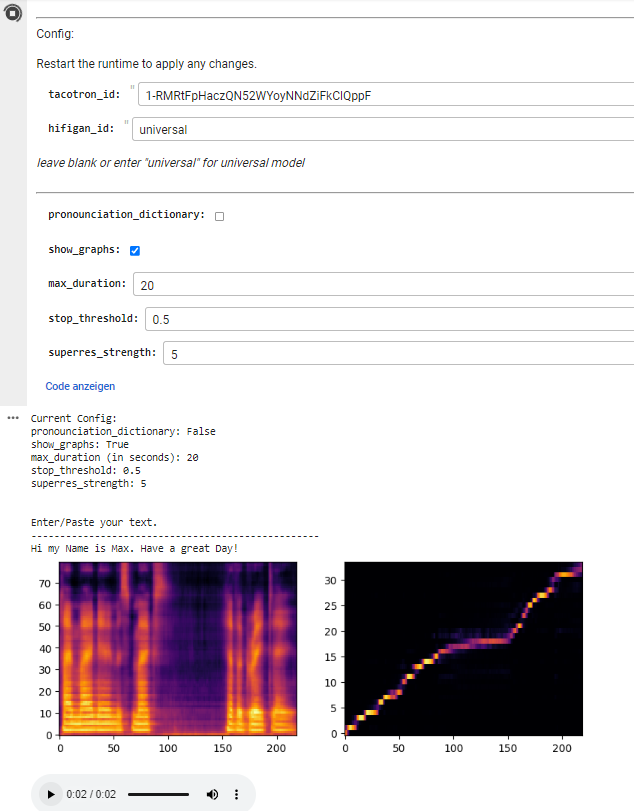
\includegraphics[width=1.0\textwidth]{Bilder/AudioTrainingSynth}
    \centering
    \caption{Synthetisierung des Modells}
    \label{fig:TrainingSynth}
\end{figure}